\documentclass{article}

\usepackage[hidelinks]{hyperref}

\usepackage{graphicx}
\graphicspath{{res/}}

\title{Interrupções e Barramento}
\author{Kinan Principe}
\date{29 abr. 2026}

\begin{document}
\maketitle
\newpage
\tableofcontents
\newpage

\section{Interrupções}
Mecanismo que interrumpe o fluxo de execução da CPU, de modo que eventos externos sejam tratados imediatamente. \newline
Essencial para sistemas multitarefa.\newline
Existem vários tipos de interrupções, a depender da origem ou resultado pretendido.

\subsection{Programa}
Ocorre durante execução de instruções e são causadas por erros ou condições especiais. Exemplos:

\begin{itemize}
    \item Divisão por zero;
    \item Instrução inválida;
    \item Acesso ilegal à memória.
\end{itemize}

\subsection{Timer}
Geradas por um \emph{temporizador interno} e permitem o controle do sistema operacional. Exemplos:

\begin{itemize}
    \item Troca de tarefas;
    \item Atualização do sistema a cada intervalo de tempo.
\end{itemize}

\subsection{Entrada/Saída}
Geradas por dispositivos externos e indicam o \emph{término} ou \emph{erro} de operação. Exemplos:

\begin{itemize}
    \item Impressora terminou a impressão;
    \item Teclado recebeu uma tecla;
    \item Disco concluiu leitura.
\end{itemize}

\subsection{Hardware}
Causadas por \emph{falhas físicas} ou \emph{problemas no sistema}. Exemplos:

\begin{itemize}
    \item Falta de energia;
    \item Erro de memória;
    \item Superaquecimento.
\end{itemize}

\subsection{Execução sem Interrupções (polling)}
Sem interrupções, um sistema deve aguardar uma operação terminar antes de começar outra, causando drástico impacto em sua eficiência.
\begin{center}
    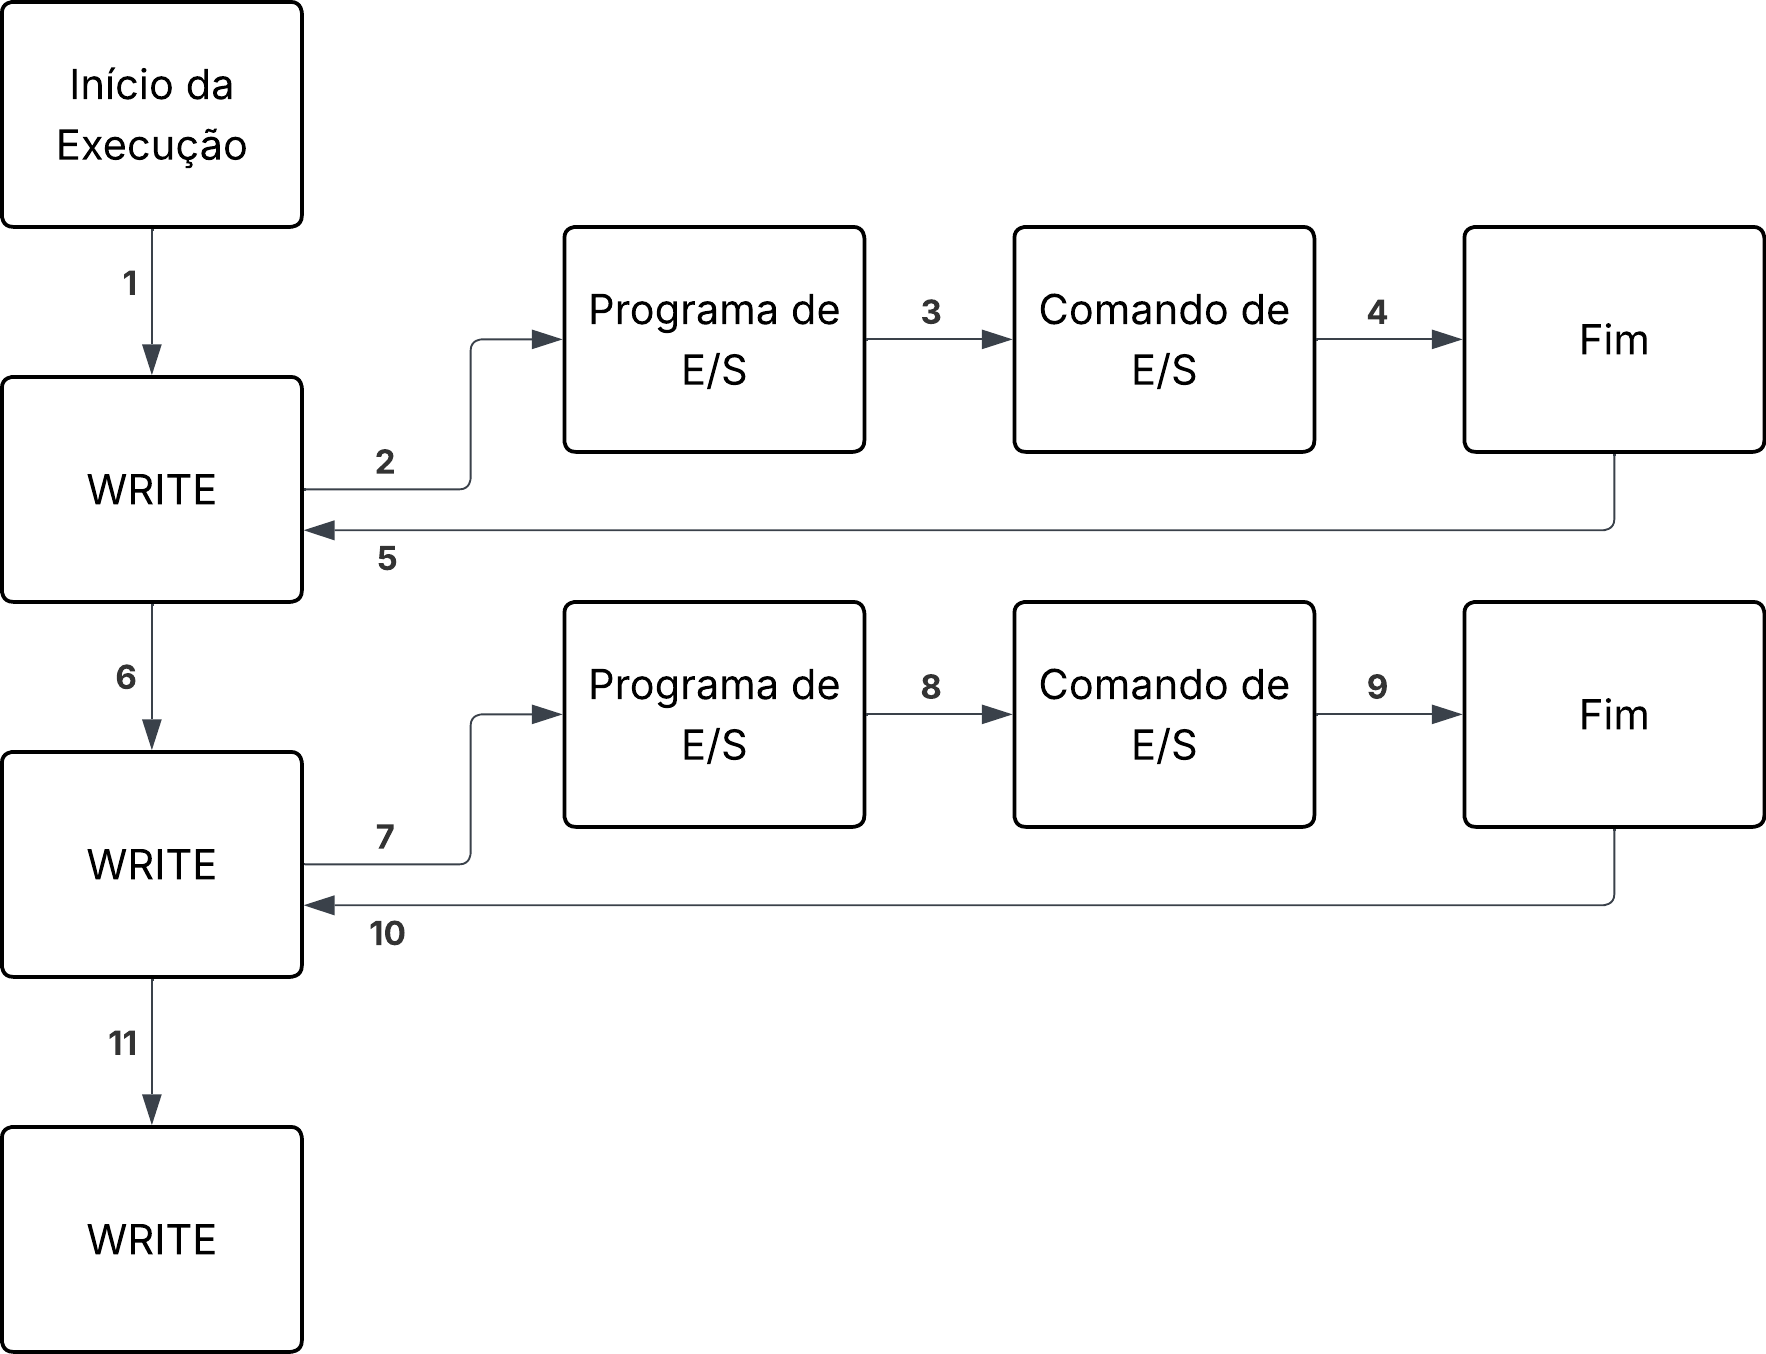
\includegraphics[scale=0.7]{execucao_sem_interrupcao}
\end{center}

\newpage
\subsection{Execução com Interrupções}
Com interrupções, um sistema inicia uma operação de entrada e saída e continua executando as outras instruções até receber uma interrupção (dispositivo sinalizando que terminou).
\begin{center}
    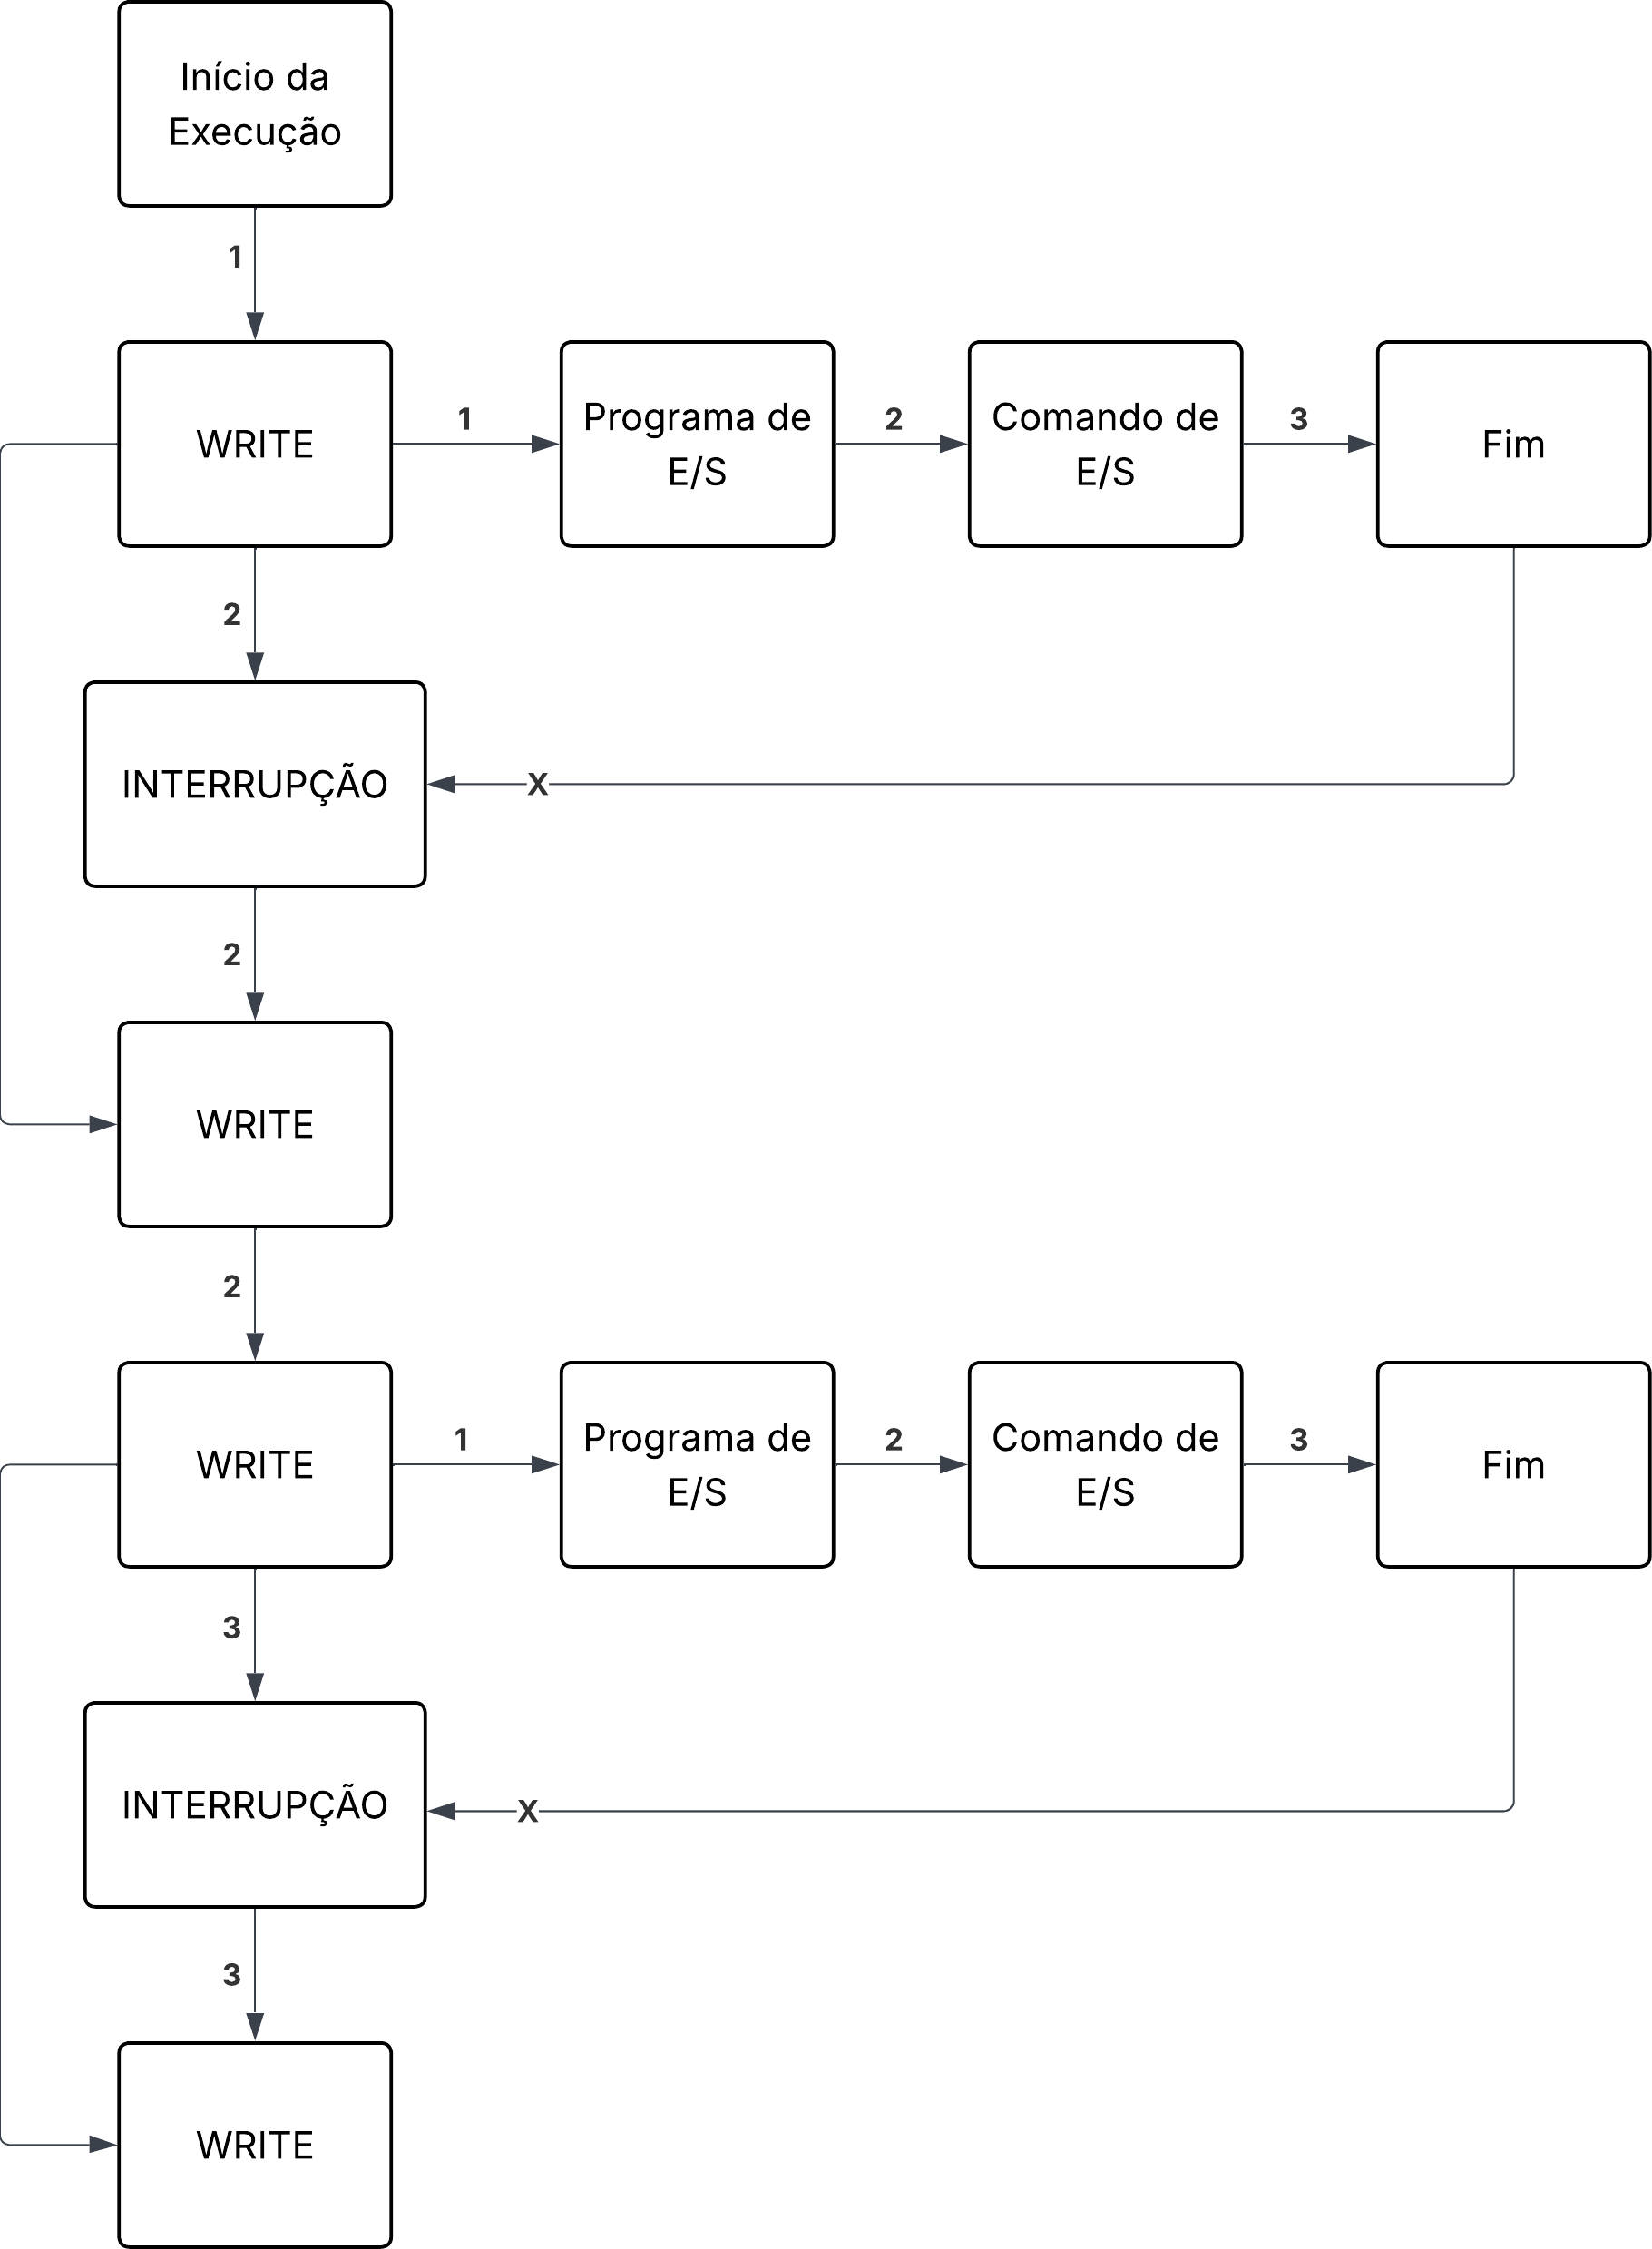
\includegraphics[scale=0.7]{execucao_com_interrupcao}
\end{center}

\section{Ciclo de Instrução com Interrupção}
O ciclo de execução das instruções com interrupções habilitadas seguem a sequência:
\begin{enumerate}
    \item Busca (fetch);
    \item Execução (execute);
    \item Verificação de interrupção.
\end{enumerate}

\begin{center}
    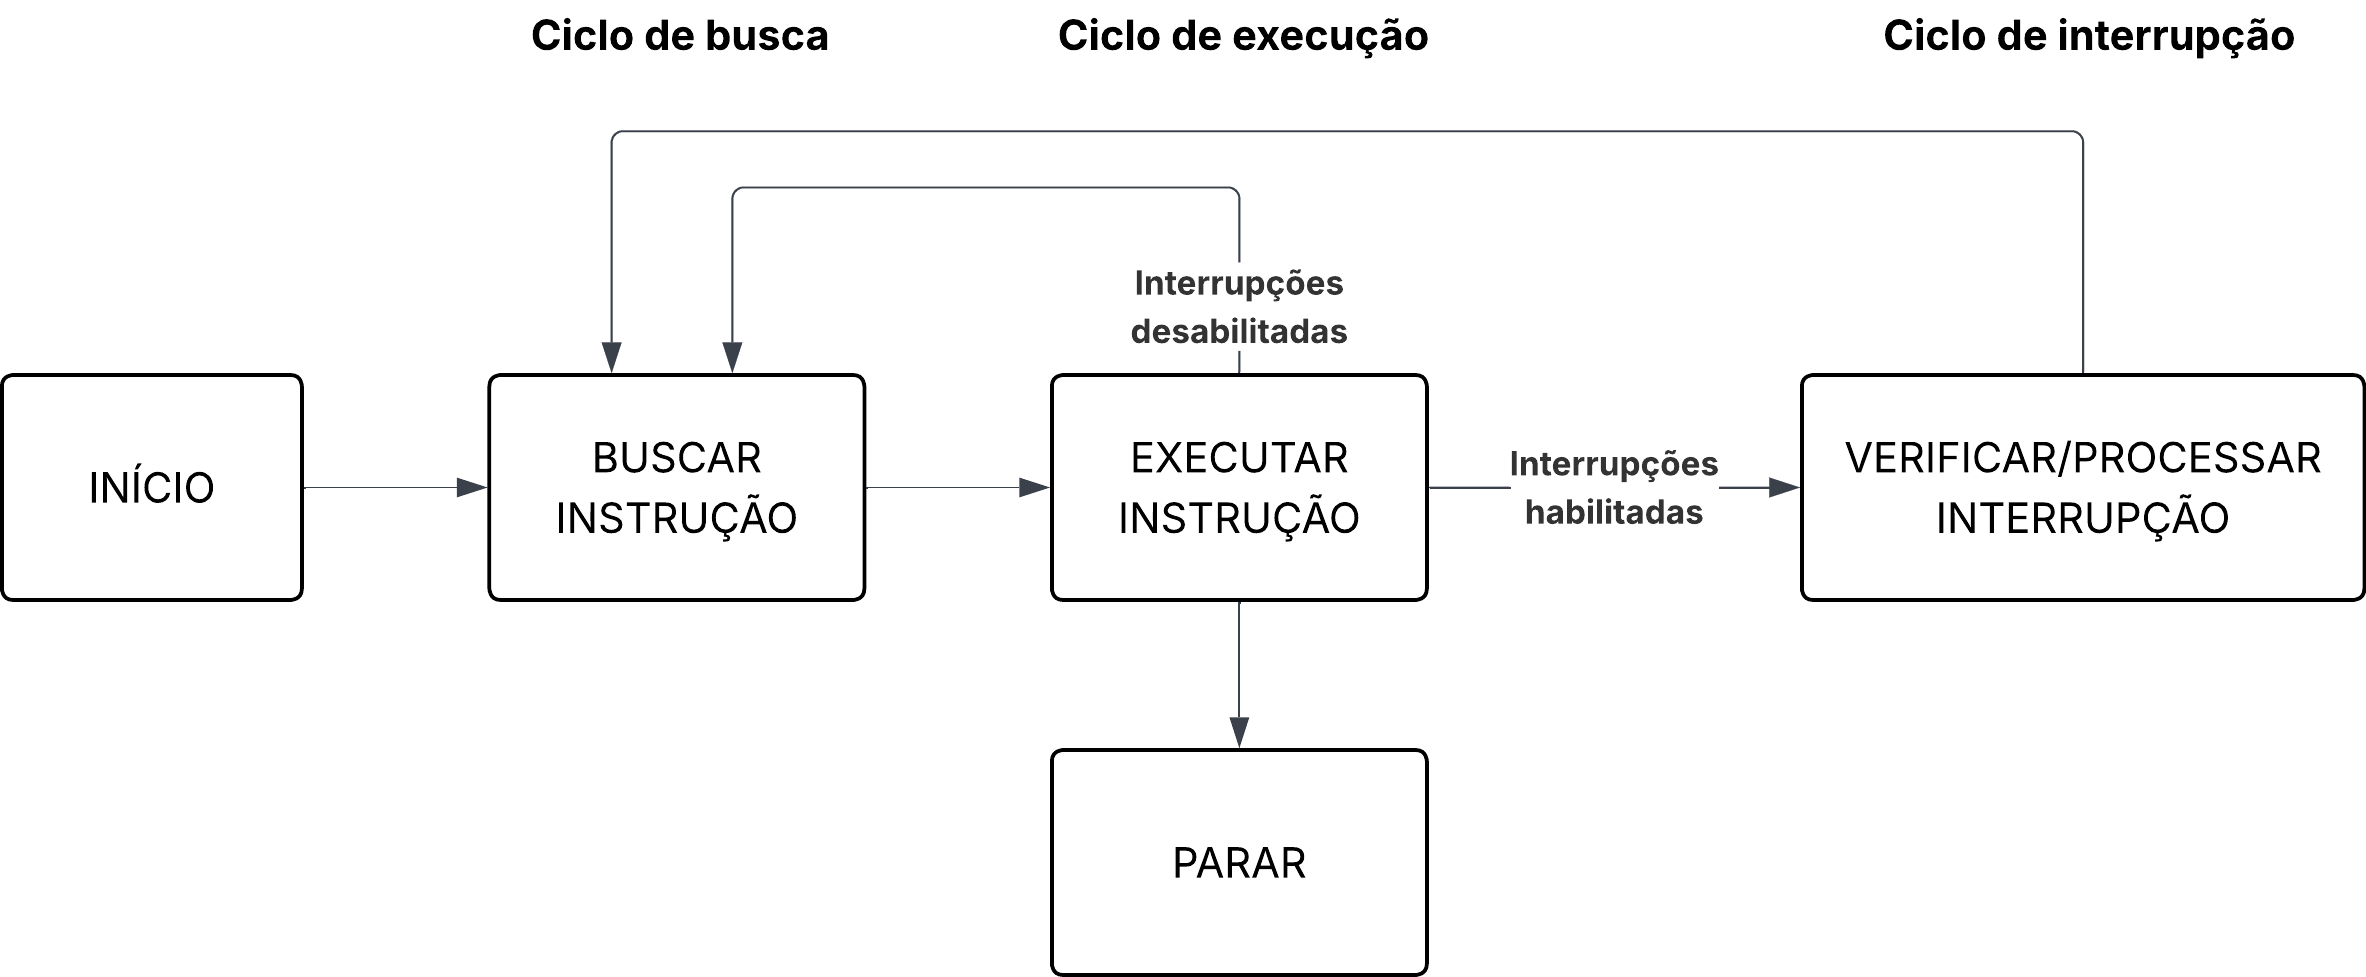
\includegraphics[scale=0.7]{ciclo_instrucao_interrupcao}
\end{center}

\subsection{Tratador de Interrupção}
Também chamado de \emph{ISR} (Interrupt Service Routine), é um código do sistema operacional que identifica a origem da interrupção e executa a ação necessária.

\subsection{Overhead}
O \emph{overhead de interrupções} é o tempo e recursos computacionais gastos para \emph{salvar contexto}, \emph{executar ISR} e \emph{restaurar o contexto}. Em suma, é o custo do uso das interrupções.

\section{Interrupções Simultâneas}
Vários dispositivos poderam gerar múltiplas interrupções ao mesmo tempo e existem diversas maneiras de como o sistema decide qual é que será efetuada.

\subsection{Por Prioridade}
Uma das maneiras é definindo para cada interrupção um nível de prioridade, podendo até determinada interrupção mais importante interromper uma outra interrupção. Exemplo:
\begin{itemize}
    \item Comunicação (alta prioridade);
    \item Disco (média prioridade);
    \item Impressora (baixa prioridade).
\end{itemize}

\section{Estrutura de Interconexão}
Conecta os seguintes componentes do sistema: \emph{CPU}, \emph{Memória} e \emph{Dispositivos de Entrada e Saída}.

\subsection{Barramento}
Conjunto de linhas paralelas, onde cada linha transporta um \emph{bit}. \newline
O barramento é um meio de comunicação compartilhado que comunica múltiplos dispositivos e permite a troca de dados entre eles. Apenas um dispositivo transimite por vez, pois senão pode gerar conflitos.
\begin{itemize}
    \item \textbf{Barramento de Dados:} Responsável por transportar dados entre \emph{CPU}, \emph{Memória} e \emph{Dispositivos de Entrada e Saída}.
    \begin{itemize}
        \item A quantidade de bits transmitidos depende da largura do barramento (8, 16, 32, 64 bits).
    \end{itemize}
    
\item \textbf{Barramento de Endereço:} Indica onde o dado deve ir/vir, ou seja, uma posição na memória ou dispositivo. Sua largura determina a capacidade máxima de memória.
    \begin{itemize}
        \item Por exemplo, um barramento de \emph{32 bits} pode endereçar até \emph{4GB} de memória.
    \end{itemize}

    \item \textbf{Barramento de Controle:} Responsável por controlar e sincronizar as operações com sinais como: \emph{READ}, \emph{WRITE}, \emph{CLOCK}, \emph{INTERRUPT}.
    \begin{itemize}
        \item A \emph{CPU} pode, por exemplo, enviar um sinal \emph{READ} para ler um determinado dado da memória.
    \end{itemize}
\end{itemize}

\subsection{Operação do Barramento}
Os sistemas computacionais fazem uso da \textit{arbitragem} para organizar o acesso ao barramento pelos dispositivos e evitar conflitos (dois ou mais dispositivos acessando o barramento simultanemanete). \\ \\
A \textit{arbitragem} ocorre como um conjunto de etapas na seguinte ordem:
\begin{enumerate}
    \item \textbf{Solicitação:} O Dispositivo pede o controle do barramento para o sistema (\emph{bus reques}).
    \item \textbf{Concessão:} O Sistema decide quem pode usar o barramento (\emph{bus grant}).

    \item \textbf{Transferência de Dados:} O Dispositivo envia:
        \begin{itemize}
            \item \textit{Endereço} (Onde acessar);
            \item \textit{Dados} (O que transferir);
            \item \textit{Controle} (leitura/escrita);
        \end{itemize}

    \item \textbf{Confirmação:} O Dispositivo destino confirma a operação com o sinal \textbf{ACK} (acknowledge).
    \item \textbf{Liberação do Barramento:} Após o uso, dispositivo libera o barramento para outro dispositivo utilizar.
\end{enumerate}

\subsection{Limitações do Barramento}
\begin{itemize}
    \item \textbf{Gargalo de Desempenho}: Apenas um dispositivo por vez pode acessá-lo e os outros devem esperar;
    \item \textbf{Concorrência e Conflitos}: Múltiplos dispositivos disputam o uso, podendo ocorrer \textit{colisão de sinais};
    \item \textbf{Escalabilidade Limitada}: Quanto mais dispositivos conectados, pior o desempenho e maior o tempo de espera.
    \item \textbf{Limitação Física e Elétrica}: Dificuldade de aumentar a velocidade e problemas de sincronização em altas frequências;
    \item \textbf{Latência maior}: O processo de solicitar acesso, aguardar liberação e realizar a operação é demorado;
\end{itemize}

\section{Principais tipos de Arbitragem}

\subsection{Arbitragem Centralizada}
Nesse modelo existe um árbitro central, que geralmente é a \emph{CPU} ou um \emph{controlador}.
\begin{itemize}
    \item \textbf{Prioridade Fixa:} Cada dispisitivo tem uma prioridade definida e o de maior prioridade sempre ganha.
        \begin{itemize}
            \item Modelo simples, no entanto, pode acarretar em \textit{starvation} em processos mais complexos, onde dispositivos de baixa prioridade podem nunca conseguirem acesso ao barramento.
        \end{itemize}

    \item \textbf{Prioridade Rotativa:} O acesso alterna entre os dispositivos.
        \begin{itemize}
            \item Justo mas não é eficiente atendendo urgências.
        \end{itemize}

    \item \textbf{Prioridade Dinâmica:} A prioridade muda com o tempo ou situação, por exemplo, dispositivos com muito tempo de espera ganham prioridade ou dispositivos críticos recebem propridade temporária.
        \begin{itemize}
            \item Modelo mais eficiente;
            \item Evita starvation.
        \end{itemize}
\end{itemize}

\subsection{Arbitragem Distribuída}
Não existe um árbitro central e os dispositivos decidem entre si.

\begin{itemize}
    \item \textbf{Auto-seleção:} Todos colocam seu identificador no barramento e o maior ou menor valor vence.
    \begin{itemize}
        \item Rápido e paralelo.
    \end{itemize}

    \item \textbf{Detecção de Colisão:} Dispositivos tentam usar o barramento e, se houver conflito, tentam novamente.
    \begin{itemize}
        \item Simples mas pode gerar atrasos.
    \end{itemize}

\item \textbf{Token Passing:} Um token (permissão) circula entre os dispositivos e só quem o tem pode acessar o barramento.
    \begin{itemize}
        \item Organizado e sem conflitos mas pode ser mais lento.
    \end{itemize}
\end{itemize}

\section{Interconexão Ponto a Ponto (Point-to-Point)}
Componentes são ligados diretamente entre si e cada conexão é dedicada.

\begin{itemize}
    \item Alta velocidade, menor latência;
    \item Maior escalabilidade;
    \item Comunicação feita por \textit{pacotes de dados}.
\end{itemize}

\textbf{Exemplos:} PCI Express (placas de vídeo, SSDs), Quick Path Interconnect - QPI (comunicação entre múltiplos processadores).

\end{document}
